\section{Submission to EMDB protocol}
\label{app:exportToEMDB}

Protocol designed to save in a specified folder main files required to submit cryo-EM derived electron density maps and derived atomic structures to EMDB, as well as other additional files that EMDB encourages to submit (\url{https://deposit-pdbe.wwpdb.org/deposition//}). Although the submission has to be performed online, this protocol tries to help the user to organize their results in different folders according to each particular submission date, project, and so on.

 \begin{itemize}
  \item \scipion menu:
  
    \ttt{Model building -> Exports} (\ffigure{fig:export_to_EMDB_1} (A))
  
  \item Protocol form parameters (\ffigure{fig:export_to_EMDB_1} (B)):
  
    \begin{figure}[H]
     \centering 
     \captionsetup{width=.9\linewidth} 
     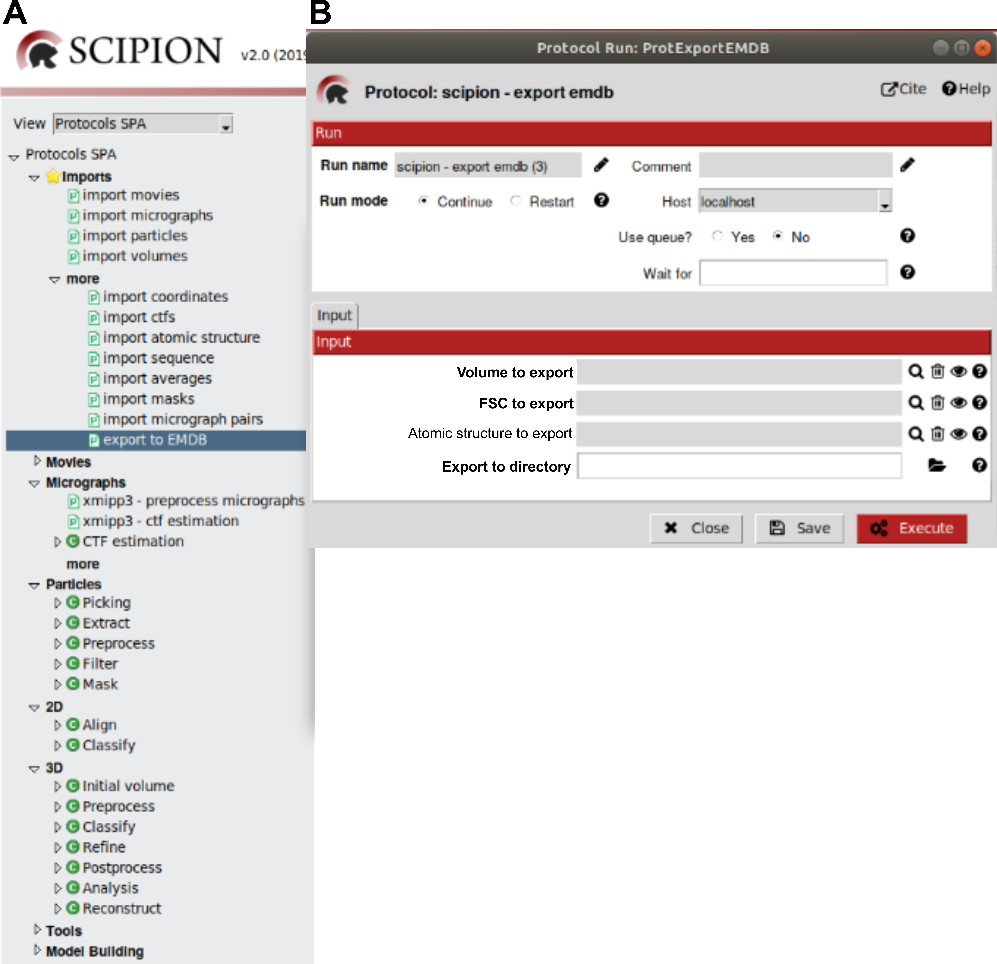
\includegraphics[width=0.90\textwidth]{Images_appendix/Fig156.pdf}
     \caption{Protocol \scommand{export to EMDB}. A: Protocol location in \scipion menu. B: Protocol form.}
     \label{fig:export_to_EMDB_1}
    \end{figure}
    
    \begin{itemize}
     \item \ttt{Input} section

    \begin{itemize}
     \item \ttt{Main EM map to export}: Param to select the electron density map previously downloaded or generated in \scipion that you would like to submit to EMDB as \ttt{main map}. The map file will be saved with \ttt{.mrc} format. If the \ttt{main map} has the two half maps associated, they will be also saved at the same time in the same directory.
     \item \ttt{Additional maps to export?}: In case you would like to submit other types of maps, specially those generated during the postprocessing like sharpening maps, select \ttt{Yes} and a new form param (\ttt{Additional EM maps to export}) will be opened to interrogate about the additional files (.mrc format). Take into account that all of them should be previously generated or imported in \scipion.
     \item \ttt{FSC to export}: Param to select the FSC file previously generated in \scipion that we would like to submit to EMDB. This file will be saved with \ttt{.xml} format.
      \item \ttt{Masks to export?}: EMDB also encourages to submit masks relevant in reconstruction or postprocessing steps. Select \ttt{Yes} if you want to include one or several masks and a new form param (\ttt{Masks to export}) will open to interrogate about the masks (.mrc format).
     \item \ttt{Atomic structure to export}: Param to select the file of coordinates from the volume-associated atomic structure previously downloaded or generated in \scipion that we would like to submit to EMDB. This file will be saved with \ttt{.cif} format.
     \item \ttt{Image to export}: Map image to represent the map in the database. 
     \item \ttt{Export to directory}: Directory specified by the user to save the three above selected files. In order to get appropriate data organization, a name related with the submission is recommended (date, project, number, ...).
    \end{itemize}
   \end{itemize}

  \item Protocol execution:
  
  Adding specific protocol label is recommended in \ttt{Run name} section, at the form top. To add the label, open the protocol form, press the pencil symbol at the right side of \ttt{Run name} box, complete the label in the new opened window, press OK and, finally, close the protocol. This label will be shown in the output summary content (see below). If you want to run again this protocol, do not forget to set to \ttt{Restart} the \ttt{Run mode}.\\
  Press the \ttt{Execute} red button at the form bottom.
  
  All the previously selected files will be saved in the chosen directory after executing the protocol and this can be checked by opening that folder. Content of the selected directory:
  \begin{itemize}
     \item \ttt{main\_map.mrc}
     \item \ttt{half\_map\_1.mrc}
     \item \ttt{half\_map\_2.mrc}
     \item Folder of additional maps: \ttt{addMaps}, which contains \ttt{map\_01.mrc, map\_02.mrc}, etc.
     \item \ttt{FSC\_file\_name.xml}
     \item Mask folder: \ttt{masks}, which contains \ttt{mask\_01, mask\_02}, etc.
     \item Input atomic structure: \ttt{atomic\_structure\_file\_name.cif/pdb}
     \item Atomic structure complete: \ttt{coordinates.cif}
     \item Atomic structure symplified: \ttt{symplified\_atom\_structure.cif}
     \item \ttt{image.png}
  \end{itemize}
  As you can see, two coordinate files have been created, complete and symplified, to try to satisfy different format demands.\\
  No additional specific visualization tools have been added to this protocol. 

  \item Summary content:
  
   The summary specifies the path to the directory selected to save the files:\\
   \ttt{Data available at: $path$}
    
\end{itemize}




